\documentclass[11pt]{report}

% Paquetes y configuraciones adicionales
\usepackage{graphicx}
\usepackage[export]{adjustbox}
\usepackage{caption}
\usepackage{float}
\usepackage{titlesec}
\usepackage{geometry}
\usepackage[hidelinks]{hyperref}
\usepackage{titling}
\usepackage{titlesec}
\usepackage{parskip}
\usepackage{wasysym}
\usepackage{tikzsymbols}
\usepackage{fancyvrb}
\usepackage{xurl}
\usepackage{hyperref}
\usepackage{subcaption}

\usepackage{listings}
\usepackage{xcolor}

\usepackage[spanish]{babel}

\newcommand{\subtitle}[1]{
  \posttitle{
    \par\end{center}
    \begin{center}\large#1\end{center}
    \vskip0.5em}
}

% Configura los márgenes
\geometry{
  left=2cm,   % Ajusta este valor al margen izquierdo deseado
  right=2cm,  % Ajusta este valor al margen derecho deseado
  top=3cm,
  bottom=3cm,
}

% Configuración de los títulos de las secciones
\titlespacing{\section}{0pt}{\parskip}{\parskip}
\titlespacing{\subsection}{0pt}{\parskip}{\parskip}
\titlespacing{\subsubsection}{0pt}{\parskip}{\parskip}

% Redefinir el formato de los capítulos y añadir un punto después del número
\makeatletter
\renewcommand{\@makechapterhead}[1]{%
  \vspace*{0\p@} % Ajusta este valor para el espaciado deseado antes del título del capítulo
  {\parindent \z@ \raggedright \normalfont
    \ifnum \c@secnumdepth >\m@ne
        \huge\bfseries \thechapter.\ % Añade un punto después del número
    \fi
    \interlinepenalty\@M
    #1\par\nobreak
    \vspace{10pt} % Ajusta este valor para el espacio deseado después del título del capítulo
  }}
\makeatother

% Configura para que cada \chapter no comience en una pagina nueva
\makeatletter
\renewcommand\chapter{\@startsection{chapter}{0}{\z@}%
    {-3.5ex \@plus -1ex \@minus -.2ex}%
    {2.3ex \@plus.2ex}%
    {\normalfont\Large\bfseries}}
\makeatother

% Configurar los colores para el código
\definecolor{codegreen}{rgb}{0,0.6,0}
\definecolor{codegray}{rgb}{0.5,0.5,0.5}
\definecolor{codepurple}{rgb}{0.58,0,0.82}
\definecolor{backcolour}{rgb}{0.95,0.95,0.92}

% Configurar el estilo para el código
\lstdefinestyle{mystyle}{
  backgroundcolor=\color{backcolour},   
  commentstyle=\color{codegreen},
  keywordstyle=\color{magenta},
  numberstyle=\tiny\color{codegray},
  stringstyle=\color{codepurple},
  basicstyle=\ttfamily\footnotesize,
  breakatwhitespace=false,         
  breaklines=true,                 
  captionpos=b,                    
  keepspaces=true,                 
  numbers=left,                    
  numbersep=5pt,                  
  showspaces=false,                
  showstringspaces=false,
  showtabs=false,                  
  tabsize=2
}

%==============================================================================
% Cosas para la documentación LateX
% % Sangría
% \setlength{\parindent}{1em}Texto

% % Quitar sangría
% \noindent

% % Punto
% \CIRCLE \ \ \textbf{Texto} \emph{algo}
% \begin{itemize}
%   \item \textbf{Negrita:} Texto
%   \item \textbf{Negrita:} Texto
% \end{itemize}

% % Introducir código
% \begin{center}
%   \begin{BVerbatim}
%     ... Código
%   \end{BVerbatim}
% \end{center}

% Poner una imagen
% \begin{figure}[H]
%   \centering
%   \includegraphics[scale=0.55]{img/}
%   \caption{Exportación de la base de datos en formato sql}
%   \label{fig:exportación de la base de datos en formato sql}
% \end{figure}

% Poner dos imágenes
% \begin{figure}[H]
%   \begin{subfigure}{0.5\textwidth}
%     \centering
%     \includegraphics[scale=0.45]{img/}
%     \caption{Texto imagen 1}
%   \end{subfigure}%
%   \begin{subfigure}{0.5\textwidth}
%     \centering
%     \includegraphics[scale=0.45]{img/}
%     \caption{Texto imagen 2}
%   \end{subfigure}
%   \caption{Texto general}
% \end{figure}

% % Poner una tabla
% \begin{table}[H]
%   \centering
%   \begin{tabular}{|c|c|c|c|}
%     \hline
%     \textbf{Campo 1} & \textbf{Campo 2} & \textbf{Campo 3} & \textbf{Campo 4} \\ \hline
%     Texto & Texto & Texto & Texto \\ \hline
%     Texto & Texto & Texto & Texto \\ \hline
%     Texto & Texto & Texto & Texto \\ \hline
%     Texto & Texto & Texto & Texto \\ \hline
%   \end{tabular}
%   \caption{Nombre de la tabla}
%   \label{tab:nombre de la tabla}
% \end{table}

% % Poner codigo de un lenguaje a partir de un archivo
% \lstset{style=mystyle}
% The next code will be directly imported from a file
% \lstinputlisting[language=Python]{code.py}

% “Texto entre comillas dobles”

%==============================================================================

\begin{document}

% Portada del informe
\title{Expresiones regulares}
\subtitle{Computabilidad y Algoritmia}
\author{Cheuk Kelly Ng Pante (alu0101364544@ull.edu.es)}
\date{01/10/2024}

\maketitle

\pagestyle{empty} % Desactiva la numeración de página para el índice

% Índice
\tableofcontents

% Nueva página
\cleardoublepage

\pagestyle{plain} % Vuelve a activar la numeración de página
\setcounter{page}{1} % Reinicia el contador de página a 1

% Secciones del informe
% Capitulo 1
\chapter{Ejercicios sobre operadores básicos}
\section{Cadenas sobre el alfabeto \texorpdfstring{$\{a, b\}$}{\{a, b\}} con longitud impar.}
\begin{itemize}
  \item \textbf{Expresión regular:} $(a|b)^*(a|b)$
    \begin{figure}[H]
      \centering
      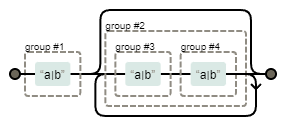
\includegraphics[scale=0.9]{img/op_basicos_01.png}
    \end{figure}
  \item \textbf{Cadenas que pertenecen al lenguaje: }
  \begin{itemize}
    \item $w_1 = a$
    \item $w_2 = aba$
    \item $w_3 = bbaba$
    \item $w_4 = aaaaaaaa$
    \item $w_5 = abababababababa$
  \end{itemize}
  \item \textbf{Cadenas que no pertenecen al lenguaje: }
  \begin{itemize}
    \item $w_6 = aa$
    \item $w_7 = abab$
    \item $w_8 = bbbbbb$
    \item $w_9 = aaaaaaaab$
    \item $w_{10} = ababababababab$
  \end{itemize}
\end{itemize}

\newpage

\section{Cadenas sobre el alfabeto \texorpdfstring{$\{a, b\}$}{\{a, b\}} con longitud igual a 5.}
\begin{itemize}
  \item \textbf{Expresión regular:} $(a|b)(a|b)(a|b)(a|b)(a|b)$
    \begin{figure}[H]
      \centering
      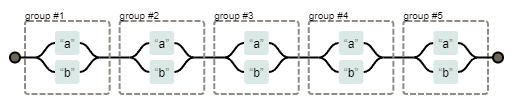
\includegraphics[scale=0.9]{img/op_basicos_02.png}
    \end{figure}
  \item \textbf{Cadenas que pertenecen al lenguaje: }
    \begin{itemize}
      \item $w_1 = aaaaa$
      \item $w_2 = bbbbb$
      \item $w_3 = ababa$
      \item $w_4 = babab$
      \item $w_5 = abbbb$
    \end{itemize}
  \item \textbf{Cadenas que no pertenecen al lenguaje: }
    \begin{itemize}
      \item $w_6 = aaaa$
      \item $w_7 = bbb$
      \item $w_8 = ababab$
      \item $w_9 = bababa$
      \item $w_{10} = abababab$
    \end{itemize}
\end{itemize}

\newpage

\section{Cadenas sobre el alfabeto \texorpdfstring{$\{a, b, c\}$}{\{a, b, c\}} con una “a” en la antepenúltima posición.}
\begin{itemize}
  \item \textbf{Expresión regular:} $(a|b|c)^*a(a|b|c)(a|b|c)$
    \begin{figure}[H]
      \centering
      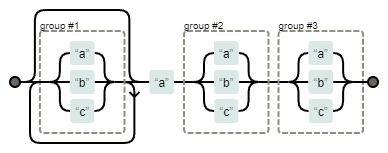
\includegraphics[scale=0.9]{img/op_basicos_03.png}
    \end{figure}
  \item \textbf{Cadenas que pertenecen al lenguaje: }
    \begin{itemize}
      \item $w_1 = abc$
      \item $w_2 = acbaabc$
      \item $w_3 = aaaaaaabb$
      \item $w_4 = abbaccbbccacaaa$
      \item $w_5 = abbbacbbbbacacb$
    \end{itemize}
  \item \textbf{Cadenas que no pertenecen al lenguaje: }
    \begin{itemize}
      \item $w_6 = a$
      \item $w_7 = bbb$
      \item $w_8 = aaaccabaabbc$
      \item $w_9 = abccdacc$
      \item $w_{10} = ababacccbabab$
    \end{itemize}
\end{itemize}

\newpage

\section{Cadenas sobre el alfabeto \texorpdfstring{$\{a, b\}$}{\{a, b\}} con número de “a”s par o número de “b”s impar.}
\begin{itemize}
  \item \textbf{Expresión regular:} $b^*(ab^*ab^*)^*|(a^*ba^*)(ba^*ba^*)^*$
    \begin{figure}[H]
      \centering
      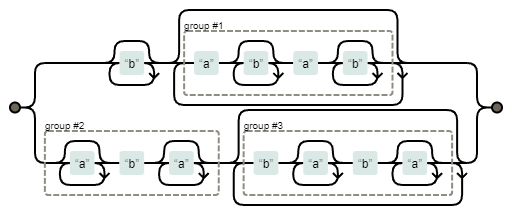
\includegraphics[scale=0.9]{img/op_basicos_04.png}
    \end{figure}
  \item \textbf{Cadenas que pertenecen al lenguaje: }
    \begin{itemize}
      \item $w_1 = baa$
      \item $w_2 = bbaa$
      \item $w_3 = bbaabbaa$
      \item $w_4 = bbaabbaabbaa$
      \item $w_5 = bbaabbaabbaabbaa$
    \end{itemize}
  \item \textbf{Cadenas que no pertenecen al lenguaje: }
    \begin{itemize}
      \item $w_6 = a$
      \item $w_7 = bb$
      \item $w_8 = abb$
      \item $w_9 = aaaaabbbbbb$
      \item $w_{10} = bbaaabb$
    \end{itemize}

\end{itemize}

\newpage

\section{Cadenas $w$ sobre el alfabeto \texorpdfstring{$\{0, 1\}$}{\{0, 1\}} tales que $2\leq |w| \leq 5$.}
\begin{itemize}
  \item \textbf{Expresión regular:} $(0|1)(0|1) \ | \ (0|1)(0|1)(0|1) \ | \ (0|1)(0|1)(0|1)(0|1) \ | \ (0|1)(0|1)(0|1)(0|1)(0|1)$
    \begin{figure}[H]
      \centering
      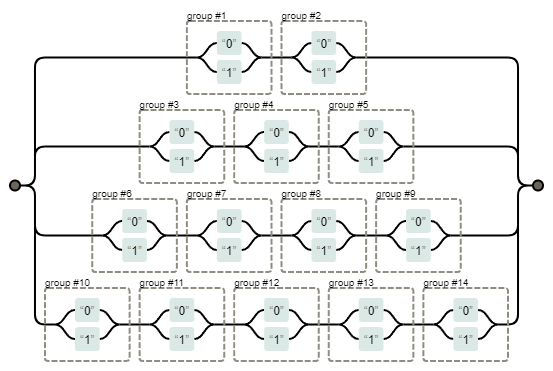
\includegraphics[scale=0.7]{img/op_basicos_05.png}
    \end{figure}
  \item \textbf{Cadenas que pertenecen al lenguaje: }
    \begin{itemize}
      \item $w_1 = 00$
      \item $w_2 = 111$
      \item $w_3 = 0011$
      \item $w_4 = 001$
      \item $w_5 = 10011$
    \end{itemize}
  \item \textbf{Cadenas que no pertenecen al el lenguaje: }
    \begin{itemize}
      \item $w_6 = 1$
      \item $w_7 = 0$
      \item $w_8 = 11001100$
      \item $w_9 = 0000000$
      \item $w_{10} = 1000101111000$
    \end{itemize}
\end{itemize}

\newpage

\section{Cadenas sobre el alfabeto \texorpdfstring{$\{0, 1\}$}{\{0, 1\}} con longitud multiplo de 3.}
\begin{itemize}
  \item \textbf{Expresión regular:} $((0|1)(0|1)(0|1))^*$
    \begin{figure}[H]
      \centering
      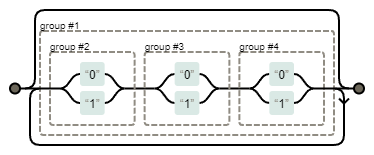
\includegraphics[scale=0.8]{img/op_basicos_06.png}
    \end{figure}
  \item \textbf{Cadenas que pertenecen al lenguaje: }
    \begin{itemize}
      \item $w_1 = 000$
      \item $w_2 = 111000$
      \item $w_3 = 101010$
      \item $w_4 = 001001001$
      \item $w_5 = 110110110110$
    \end{itemize}
  \item \textbf{Cadenas que no pertenecen al lenguaje: }
    \begin{itemize}
      \item $w_6 = 0$
      \item $w_7 = 11$
      \item $w_8 = 1010$
      \item $w_9 = 00111$
      \item $w_{10} = 1001001$
    \end{itemize}
\end{itemize}

\newpage

\section{Cadenas sobre el alfabeto \texorpdfstring{$\{0, 1\}$}{\{0, 1\}} con una longitud que no sea múltiplo de 3.}
\begin{itemize}
  \item \textbf{Expresión regular:} $((0|1)(0|1)(0|1))^*(0|1)|(0|1)(0|1)$
    \begin{figure}[H]
      \centering
      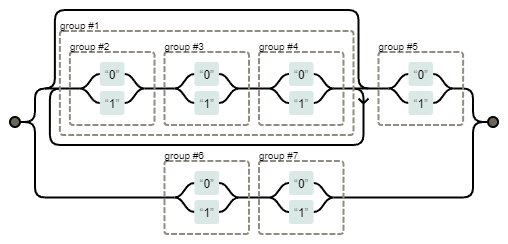
\includegraphics[scale=0.9]{img/op_basicos_07.png}
    \end{figure}
  \item \textbf{Cadenas que pertenecen al lenguaje: }
    \begin{itemize}
      \item $w_1 = 0$
      \item $w_2 = 1$
      \item $w_3 = 00$
      \item $w_4 = 1100$
      \item $w_5 = 0000110$
    \end{itemize}
  \item \textbf{Cadenas que no pertenecen al lenguaje: }
    \begin{itemize}
      \item $w_6 = 000$
      \item $w_7 = 111000$
      \item $w_8 = 101010$
      \item $w_9 = 001001001$
      \item $w_{10} = 110110110110$
    \end{itemize}
\end{itemize}

\newpage

\section{Cadenas $w$ sobre el alfabeto \texorpdfstring{$\{0, 1\}$}{\{0, 1\}} tal que $w = 0^n1^m$ con $n + m$ impar.}
\begin{itemize}
  \item \textbf{Expresión regular:} $(0(00)^*)(11(11)^*)|(00(00)^*)(1(11)^*)$
    \begin{figure}[H]
      \centering
      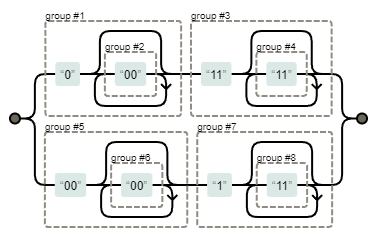
\includegraphics[scale=0.9]{img/op_basicos_08.png}
    \end{figure}
  \item \textbf{Cadenas que pertenecen al lenguaje: }
    \begin{itemize}
      \item $w_1 = 01$
      \item $w_2 = 000111$
      \item $w_3 = 0000111$
      \item $w_4 = 000001111$
      \item $w_5 = 00000011111$
    \end{itemize}
  \item \textbf{Cadenas que no pertenecen al lenguaje: }
    \begin{itemize}
      \item $w_6 = 0$
      \item $w_7 = 1$
      \item $w_8 = 0000$
      \item $w_9 = 1111$
      \item $w_{10} = 000011$
    \end{itemize}
\end{itemize}

\newpage

\section{Cadenas sobre el alfabeto \texorpdfstring{$\{0,1,2,3,4,5,6,7,8,9\}$}{\{0,1,2,3,4,5,6,7,8,9\}} que tengan como máximo dos ceros.}
\begin{itemize}
  \item \textbf{Expresión regular:} $(1|2|3|4|5|6|7|8|9)^*|(1|2|3|4|5|6|7|8|9)^*0(1|2|3|4|5|6|7|8|9)^*|$ \newline $(1|2|3|4|5|6|7|8|9)^*0(1|2|3|4|5|6|7|8|9)^*0(1|2|3|4|5|6|7|8|9)^*$
    \begin{figure}[H]
      \centering
      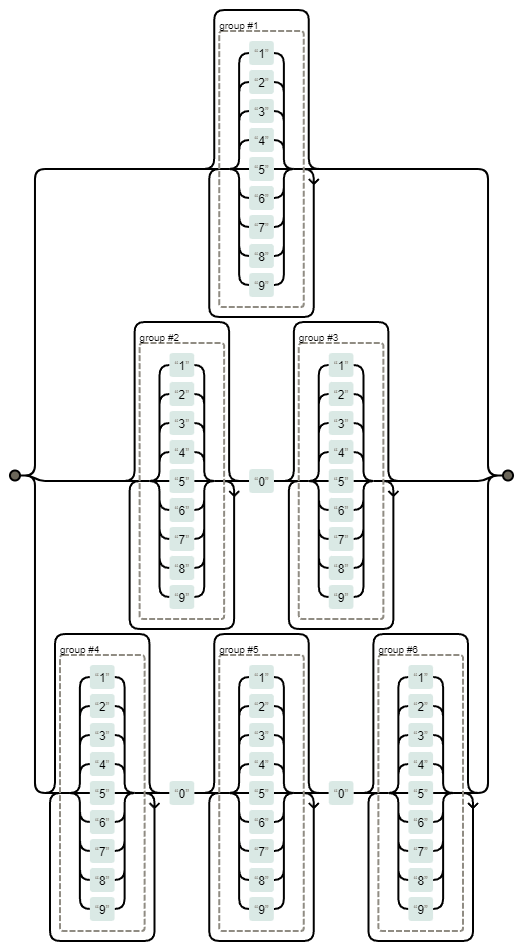
\includegraphics[scale=0.5]{img/op_basicos_09.png}
    \end{figure}
    \newpage
  \item \textbf{Cadenas que pertenecen al lenguaje: }
    \begin{itemize}
      \item $w_1 = 0$
      \item $w_2 = 00$
      \item $w_3 = 012310$
      \item $w_4 = 28720099172$
      \item $w_5 = 123987087871230$
    \end{itemize}
  \item \textbf{Cadenas que no pertenecen al lenguaje: }
    \begin{itemize}
      \item $w_6 = 000$
      \item $w_7 = 013208780$
      \item $w_8 = 023001003$
      \item $w_9 = 0289000000134$
      \item $w_{10} = 00788432100$
    \end{itemize}
\end{itemize}

\newpage

\section{Cadenas sobre el alfabeto \texorpdfstring{$\{x,y,z\}$}{\{x,y,z\}} que no contenga dos símbolos x consecutivos.}
\begin{itemize}
  \item \textbf{Expresión regular:} $(x|y|z)(y|z)^+(x|y|z)$
    \begin{figure}[H]
      \centering
      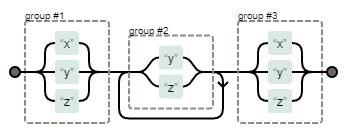
\includegraphics[scale=0.9]{img/op_basicos_10.png}
    \end{figure}
  \item \textbf{Cadenas que pertenecen al lenguaje: }
    \begin{itemize}
      \item $w_1 = x$
      \item $w_2 = xyz$
      \item $w_3 = yzzzzy$
      \item $w_4 = xzzzy$
      \item $w_5 = zy$
    \end{itemize}
  \item \textbf{Cadenas que no pertenecen al lenguaje: }
    \begin{itemize}
      \item $w_6 = xx$
      \item $w_7 = xyx$
      \item $w_8 = zxx$
      \item $w_9 = yxx$
      \item $w_{10} = zxyx$
    \end{itemize}
\end{itemize}

\newpage

\chapter{Ejercicios sobre operadores extendidos}
\section{Direcciones de correos electrónicos de estudiantes de la Universidad de La Laguna.}
\textbf{Expresión regular:} \verb|^alu\d{10}@ull\.edu\.es$|
  \begin{figure}[H]
    \centering
    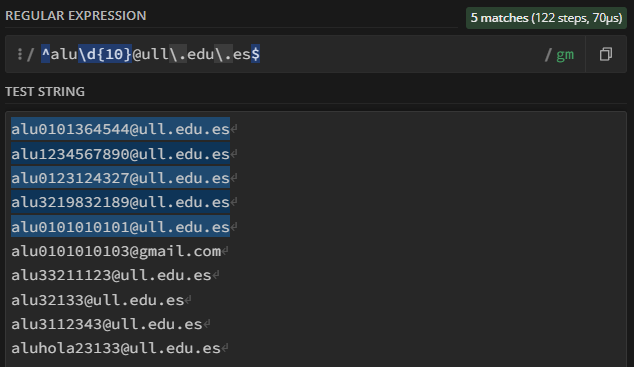
\includegraphics[scale=0.67]{img/op_extendidos_01.png}
  \end{figure}

\section{Palabras que terminen por una vocal.}
\textbf{Expresión regular:} \verb|^[a-zA-Z]*[aeiouAEIOU]$|
  \begin{figure}[H]
    \centering
    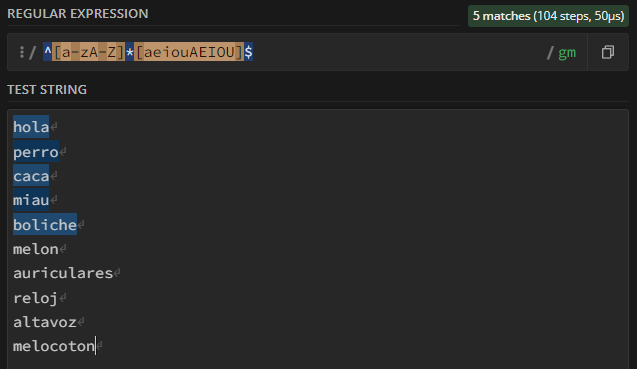
\includegraphics[scale=0.75]{img/op_extendidos_02.png}
  \end{figure}

\newpage

\section{Números enteros.}
\textbf{Expresión regular:} \verb|^[+-]?\d+$|
  \begin{figure}[H]
    \centering
    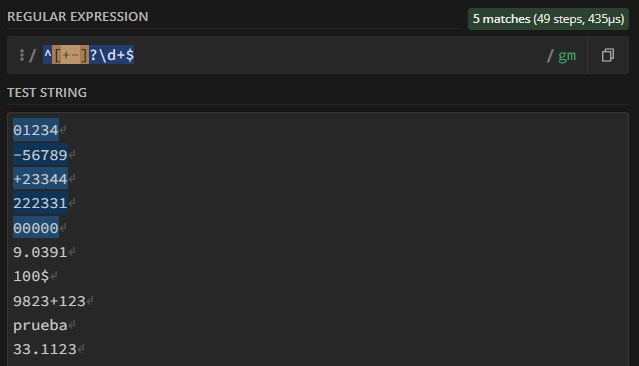
\includegraphics[scale=0.75]{img/op_extendidos_03.png}
  \end{figure}

\section{Texto que se encuentre entre paréntesis.}
\textbf{Expresión regular:} \verb|\(.*\)|
  \begin{figure}[H]
    \centering
    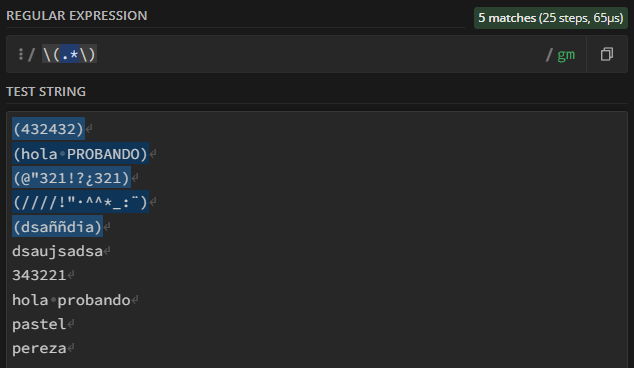
\includegraphics[scale=0.75]{img/op_extendidos_04.png}
  \end{figure}

\newpage

\section{Código postal en España.}
\textbf{Expresión regular:}
\begin{verbatim}
^(0[1-9]\d{3}|\[1-4]\d{4}|\5[0-2]\d{3})$
\end{verbatim}
\begin{figure}[H]
  \centering
  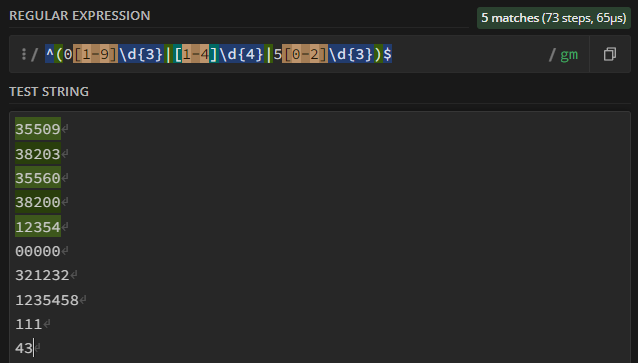
\includegraphics[scale=0.75]{img/op_extendidos_05.png}
\end{figure}

\section{Palabras que contienen solo letras mayúsculas.}
\textbf{Expresión regular:} \verb|^(?=.*[A-Z])[a-zA-Z]+$|
  \begin{figure}[H]
    \centering
    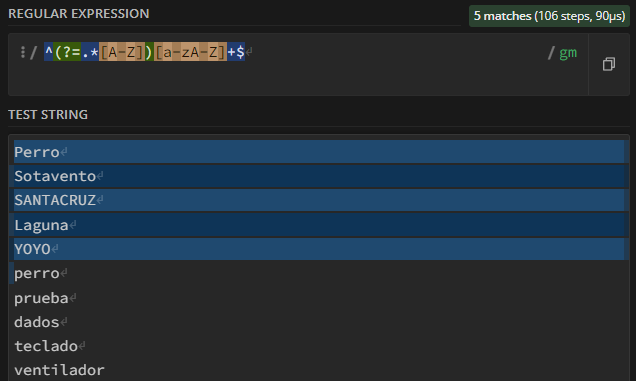
\includegraphics[scale=0.75]{img/op_extendidos_06.png} 
  \end{figure}

\newpage

\section{Número de teléfono en formato \texttt{prefijo XXX-XXX-XXX}, donde el prefijo del país puede indicarse empezando por 00 o bien con un símbolo \texttt{+}; por ejemplo, 0034 o +34 para España.}
\textbf{Expresión regular:} \texttt{\textasciicircum(00|\textbackslash+)\textbackslash d\{1,3\}-\textbackslash d\{3\}-\textbackslash d\{3\}-\textbackslash d\{3\}\$}
  \begin{figure}[H]
    \centering
    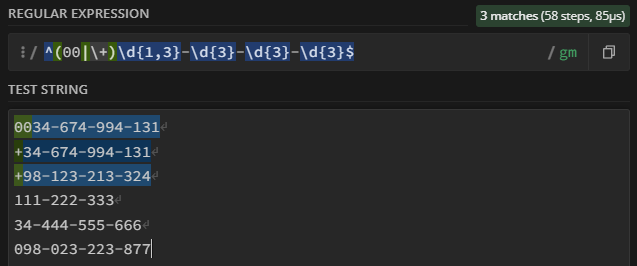
\includegraphics[scale=0.75]{img/op_extendidos_07.png}
  \end{figure}

\section{Fecha en formato \texttt{DD/MM/AAAA}.}
\textbf{Expresión regular:}
\begin{verbatim}
^(0[1-9]|[12][0-9]|3[01])\/(0[1-9]|1[0-2])\/[0-9]{4}$
\end{verbatim}
  \begin{figure}[H]
    \centering
    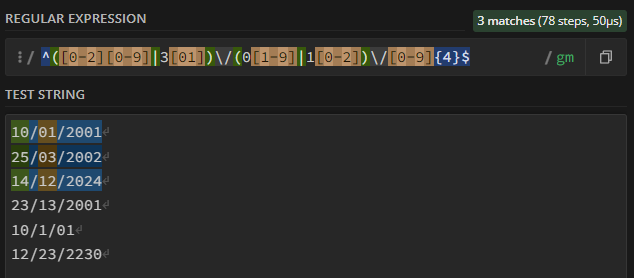
\includegraphics[scale=0.75]{img/op_extendidos_08.png}
  \end{figure}

\newpage

\section{Palabras de al menos 10 letras de longitud.}
\textbf{Expresión regular:} \verb|^[a-zA-Z]{10,}$|
  \begin{figure}[H]
    \centering
    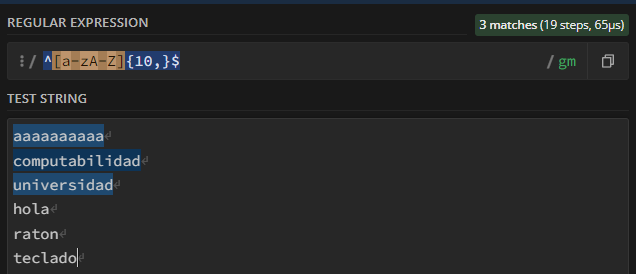
\includegraphics[scale=0.75]{img/op_extendidos_09.png}
  \end{figure}

\section{Palabras que terminen con “ing” o “ed”.}
\textbf{Expresión regular:} 
  \begin{figure}[H]
    \centering
    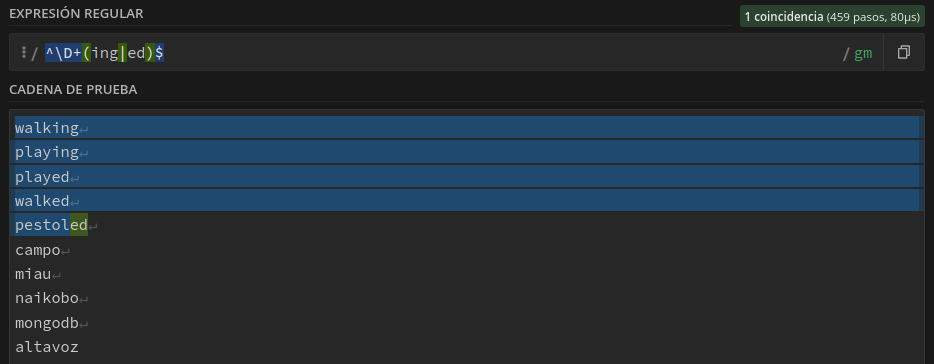
\includegraphics[scale=0.75]{img/op_extendidos_10.png}
  \end{figure}

\end{document}